\documentclass[border=10pt]{standalone}
\usepackage{tikz}
\usetikzlibrary{shapes.geometric, arrows.meta, positioning, fit, backgrounds, calc, decorations.pathmorphing, shadows.blur}

% Color palette
\definecolor{iotgreen}{HTML}{2E7D32}
\definecolor{mqttblue}{HTML}{1565C0}
\definecolor{protonest}{HTML}{6A1B9A}
\definecolor{backendorange}{HTML}{E65100}
\definecolor{dborange}{HTML}{BF360C}
\definecolor{aicolor}{HTML}{00838F}
\definecolor{mobileblue}{HTML}{0277BD}
\definecolor{layerbg1}{HTML}{E8F5E9}
\definecolor{layerbg2}{HTML}{E3F2FD}
\definecolor{layerbg3}{HTML}{FFF3E0}
\definecolor{layerbg4}{HTML}{E0F7FA}
\definecolor{layerbg5}{HTML}{E1F5FE}
\definecolor{arrowgray}{HTML}{455A64}

\begin{document}
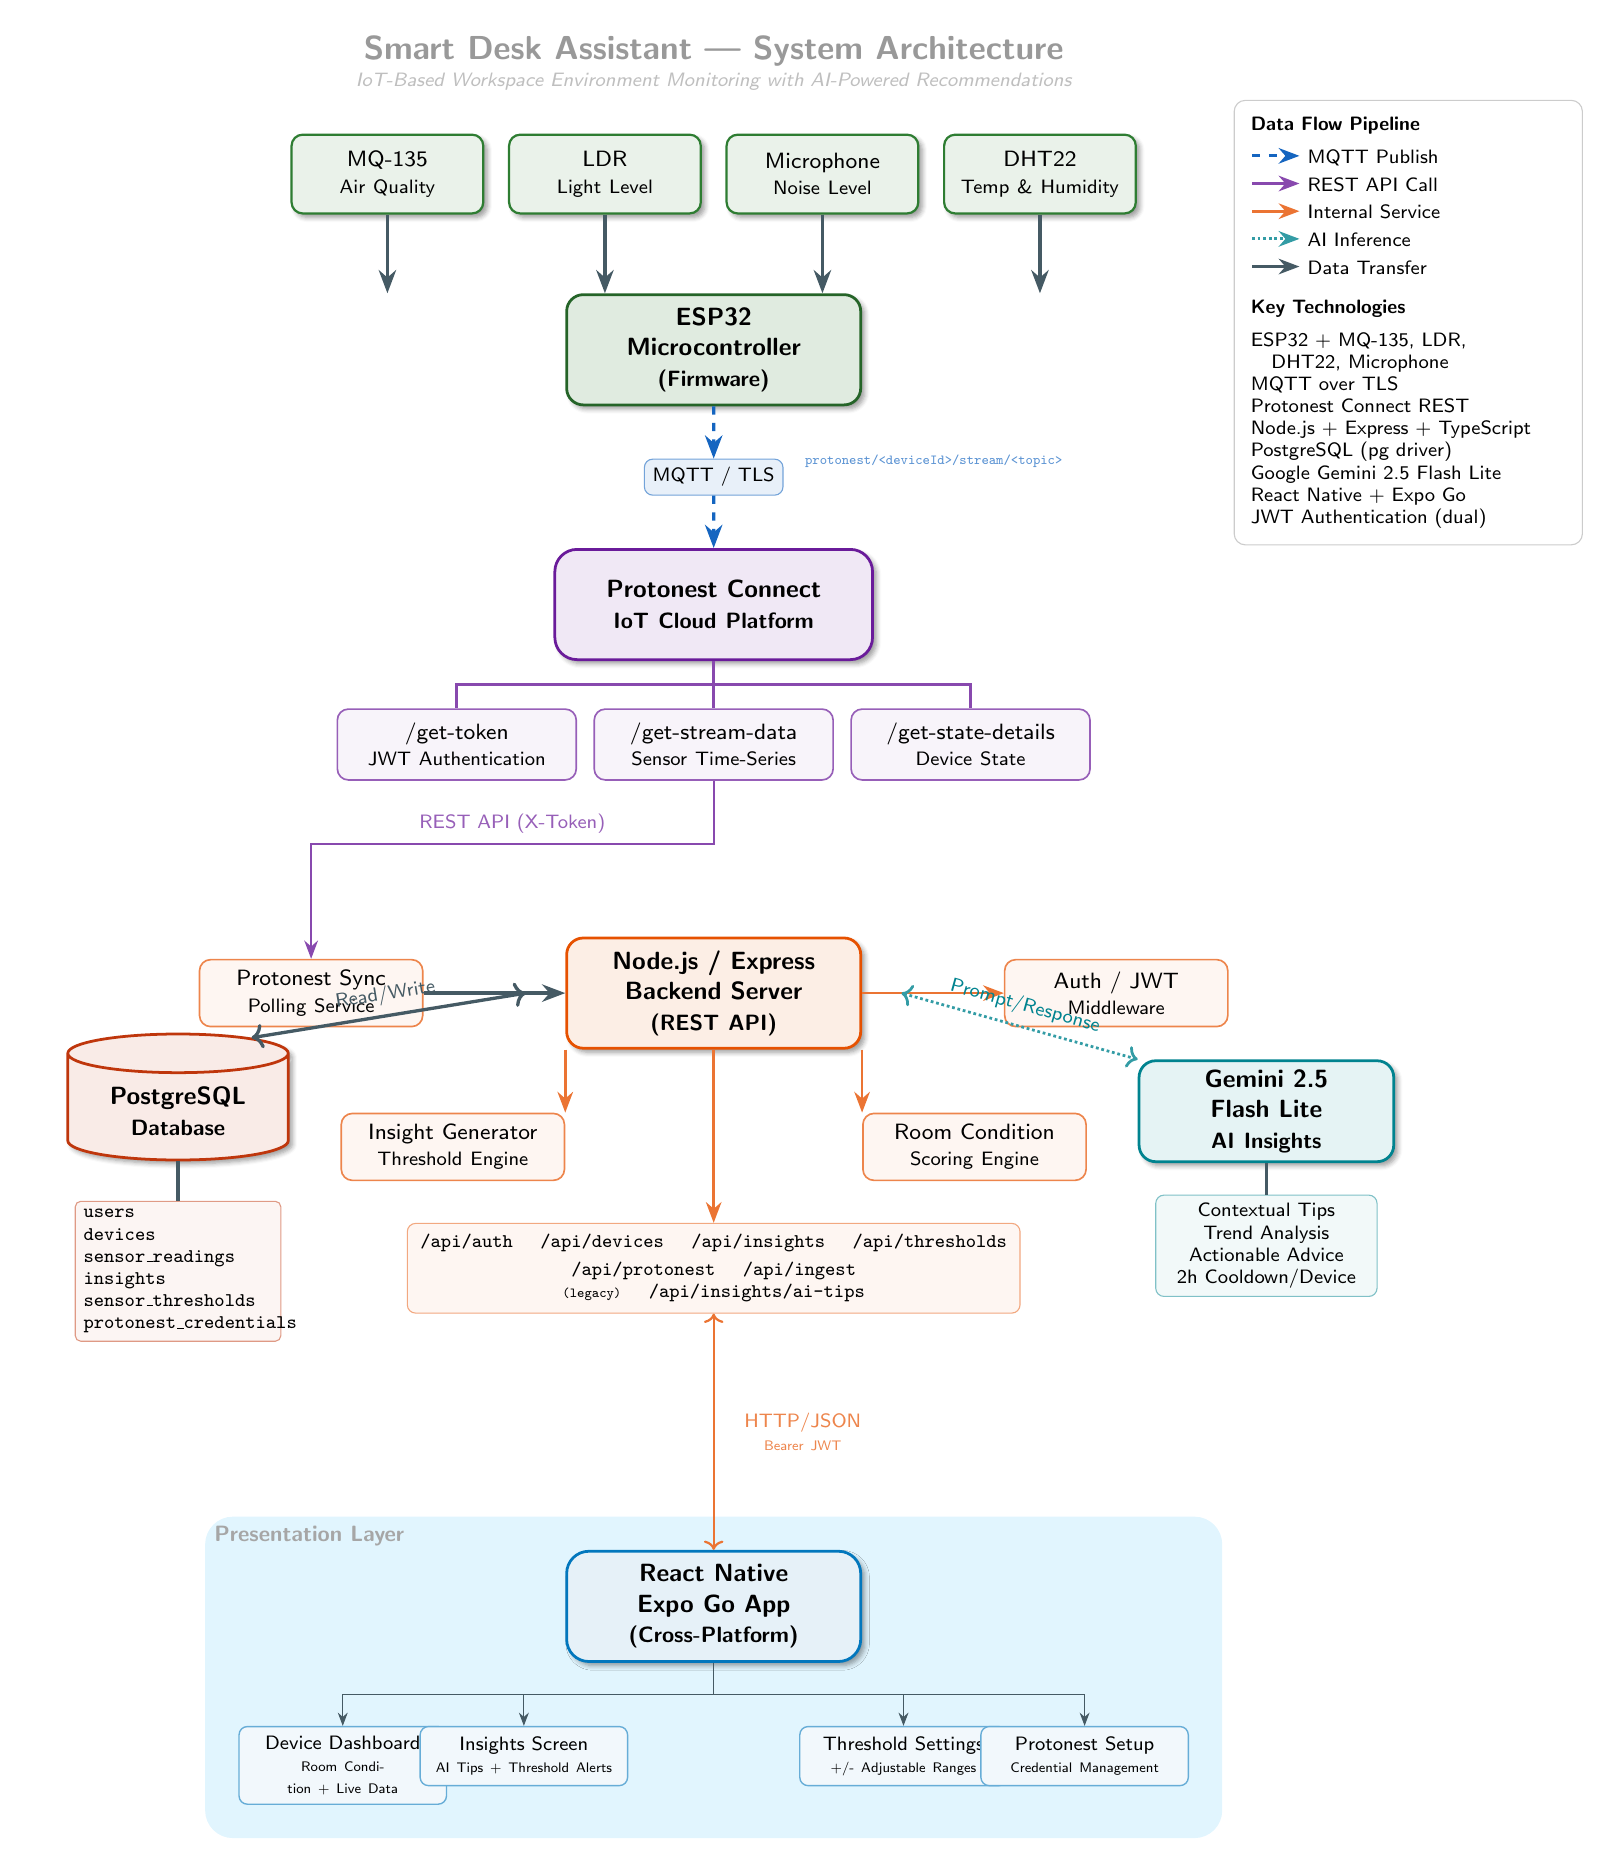
\begin{tikzpicture}[
    % Node styles
    sensor/.style={
        rectangle, rounded corners=4pt, draw=iotgreen, fill=iotgreen!10,
        text width=2.2cm, minimum height=1cm, align=center,
        font=\footnotesize\sffamily, line width=0.8pt,
        blur shadow={shadow blur steps=5, shadow xshift=0.5mm, shadow yshift=-0.5mm}
    },
    mcu/.style={
        rectangle, rounded corners=6pt, draw=iotgreen!80!black, fill=iotgreen!15,
        text width=3.5cm, minimum height=1.4cm, align=center,
        font=\small\sffamily\bfseries, line width=1pt,
        blur shadow={shadow blur steps=5, shadow xshift=0.5mm, shadow yshift=-0.5mm}
    },
    cloud/.style={
        rectangle, rounded corners=8pt, draw=protonest, fill=protonest!10,
        text width=3.8cm, minimum height=1.4cm, align=center,
        font=\small\sffamily\bfseries, line width=1pt,
        blur shadow={shadow blur steps=5, shadow xshift=0.5mm, shadow yshift=-0.5mm}
    },
    cloudapi/.style={
        rectangle, rounded corners=4pt, draw=protonest!70, fill=protonest!5,
        text width=2.8cm, minimum height=0.9cm, align=center,
        font=\footnotesize\sffamily, line width=0.6pt
    },
    backend/.style={
        rectangle, rounded corners=6pt, draw=backendorange, fill=backendorange!10,
        text width=3.5cm, minimum height=1.4cm, align=center,
        font=\small\sffamily\bfseries, line width=1pt,
        blur shadow={shadow blur steps=5, shadow xshift=0.5mm, shadow yshift=-0.5mm}
    },
    service/.style={
        rectangle, rounded corners=4pt, draw=backendorange!70, fill=backendorange!5,
        text width=2.6cm, minimum height=0.85cm, align=center,
        font=\footnotesize\sffamily, line width=0.6pt
    },
    database/.style={
        cylinder, shape border rotate=90, draw=dborange, fill=dborange!10,
        minimum width=2.8cm, minimum height=1.6cm, align=center,
        font=\small\sffamily\bfseries, line width=1pt,
        aspect=0.25,
        blur shadow={shadow blur steps=5, shadow xshift=0.5mm, shadow yshift=-0.5mm}
    },
    aibox/.style={
        rectangle, rounded corners=6pt, draw=aicolor, fill=aicolor!10,
        text width=3cm, minimum height=1.2cm, align=center,
        font=\small\sffamily\bfseries, line width=1pt,
        blur shadow={shadow blur steps=5, shadow xshift=0.5mm, shadow yshift=-0.5mm}
    },
    mobile/.style={
        rectangle, rounded corners=8pt, draw=mobileblue, fill=mobileblue!10,
        text width=3.5cm, minimum height=1.4cm, align=center,
        font=\small\sffamily\bfseries, line width=1pt,
        blur shadow={shadow blur steps=5, shadow xshift=0.5mm, shadow yshift=-0.5mm}
    },
    screen/.style={
        rectangle, rounded corners=3pt, draw=mobileblue!60, fill=mobileblue!5,
        text width=2.4cm, minimum height=0.75cm, align=center,
        font=\scriptsize\sffamily, line width=0.5pt
    },
    % Arrow styles
    dataarrow/.style={
        -Stealth, line width=1.2pt, color=arrowgray
    },
    mqttarrow/.style={
        -Stealth, line width=1.2pt, color=mqttblue, dashed
    },
    restarrow/.style={
        -Stealth, line width=1pt, color=protonest!80
    },
    apiarrow/.style={
        -Stealth, line width=1pt, color=backendorange!80
    },
    aiarrow/.style={
        -Stealth, line width=1pt, color=aicolor!80, densely dotted
    },
    % Layer label style
    layerlabel/.style={
        font=\footnotesize\sffamily\bfseries\itshape, text=gray!70
    }
]

% ============================================================
% LAYER 1: IoT / Perception Layer
% ============================================================

% Sensors
\node[sensor] (s_aqi) at (0, 0) {MQ-135\\{\scriptsize Air Quality}};
\node[sensor, right=0.3cm of s_aqi] (s_ldr) {LDR\\{\scriptsize Light Level}};
\node[sensor, right=0.3cm of s_ldr] (s_mic) {Microphone\\{\scriptsize Noise Level}};
\node[sensor, right=0.3cm of s_mic] (s_dht) {DHT22\\{\scriptsize Temp \& Humidity}};

% ESP32
\node[mcu, below=1cm of $(s_ldr.south)!0.5!(s_mic.south)$] (esp32) {ESP32\\Microcontroller\\{\footnotesize\itshape (Firmware)}};

% Sensor arrows
\draw[dataarrow] (s_aqi.south) -- (s_aqi.south |- esp32.north);
\draw[dataarrow] (s_ldr.south) -- (s_ldr.south |- esp32.north);
\draw[dataarrow] (s_mic.south) -- (s_mic.south |- esp32.north);
\draw[dataarrow] (s_dht.south) -- (s_dht.south |- esp32.north);

% Layer 1 background
\begin{scope}[on background layer]
    \node[fit=(s_aqi)(s_dht)(esp32), fill=layerbg1, rounded corners=10pt, inner sep=12pt] (layer1bg) {};
    \node[layerlabel, anchor=north west] at (layer1bg.north west) {Perception Layer};
\end{scope}

% ============================================================
% LAYER 2: Communication Layer (MQTT + Protonest)
% ============================================================

\node[cloud, below=1.8cm of esp32] (protonest) {Protonest Connect\\{\footnotesize IoT Cloud Platform}};

% MQTT protocol label
\node[rectangle, rounded corners=3pt, draw=mqttblue!60, fill=mqttblue!10,
      font=\scriptsize\sffamily, inner sep=3pt]
      (mqtt_label) at ($(esp32.south)!0.5!(protonest.north)$) {MQTT / TLS};

% Protonest API endpoints
\node[cloudapi, below left=0.6cm and -0.3cm of protonest] (api_token) {/get-token\\{\scriptsize JWT Authentication}};
\node[cloudapi, below=0.6cm of protonest] (api_stream) {/get-stream-data\\{\scriptsize Sensor Time-Series}};
\node[cloudapi, below right=0.6cm and -0.3cm of protonest] (api_state) {/get-state-details\\{\scriptsize Device State}};

% MQTT arrow
\draw[mqttarrow] (esp32.south) -- (mqtt_label.north);
\draw[mqttarrow] (mqtt_label.south) -- (protonest.north);

% Topic labels
\node[font=\tiny\ttfamily, color=mqttblue!70, anchor=west] at ($(mqtt_label.east)+(0.15,0.2)$)
    {protonest/<deviceId>/stream/<topic>};

% API arrows from Protonest
\draw[restarrow, -] (protonest.south) -- ++(0,-0.3) -| (api_token.north);
\draw[restarrow, -] (protonest.south) -- (api_stream.north);
\draw[restarrow, -] (protonest.south) -- ++(0,-0.3) -| (api_state.north);

% Layer 2 background
\begin{scope}[on background layer]
    \node[fit=(protonest)(api_token)(api_stream)(api_state)(mqtt_label),
          fill=layerbg2, rounded corners=10pt, inner sep=12pt] (layer2bg) {};
    \node[layerlabel, anchor=north west] at (layer2bg.north west) {Communication Layer};
\end{scope}

% ============================================================
% LAYER 3: Application Layer (Backend)
% ============================================================

\node[backend, below=3.5cm of protonest] (backend) {Node.js / Express\\Backend Server\\{\footnotesize\itshape (REST API)}};

% Backend services
\node[service, left=1.8cm of backend] (svc_sync) {Protonest Sync\\{\scriptsize Polling Service}};
\node[service, below left=0.8cm and 0cm of backend] (svc_insight) {Insight Generator\\{\scriptsize Threshold Engine}};
\node[service, below right=0.8cm and 0cm of backend] (svc_room) {Room Condition\\{\scriptsize Scoring Engine}};
\node[service, right=1.8cm of backend] (svc_auth) {Auth / JWT\\{\scriptsize Middleware}};

% Backend API routes
\node[rectangle, rounded corners=3pt, draw=backendorange!50, fill=backendorange!5,
      text width=7.5cm, align=center, font=\scriptsize\ttfamily, inner sep=4pt,
      below=2.2cm of backend]
      (routes) {
    /api/auth \quad /api/devices \quad /api/insights \quad /api/thresholds\\[2pt]
    /api/protonest \quad /api/ingest {\tiny(legacy)} \quad /api/insights/ai-tips
};

% Database
\node[database, left=3.5cm of backend, yshift=-1.5cm] (db) {PostgreSQL\\{\footnotesize Database}};

% DB tables
\node[rectangle, rounded corners=2pt, draw=dborange!50, fill=dborange!5,
      font=\scriptsize\ttfamily, text width=2.4cm, align=left, inner sep=3pt,
      below=0.5cm of db] (tables) {
    users\\
    devices\\
    sensor\_readings\\
    insights\\
    sensor\_thresholds\\
    protonest\_credentials
};

% AI Service
\node[aibox, right=3.5cm of backend, yshift=-1.5cm] (ai) {Gemini 2.5\\Flash Lite\\{\footnotesize AI Insights}};

\node[rectangle, rounded corners=3pt, draw=aicolor!50, fill=aicolor!5,
      font=\scriptsize\sffamily, text width=2.6cm, align=center, inner sep=3pt,
      below=0.4cm of ai] (ai_features) {
    Contextual Tips\\
    Trend Analysis\\
    Actionable Advice\\
    2h Cooldown/Device
};

% Arrows: Protonest → Backend
\draw[restarrow, thick] (api_stream.south) -- ++(0,-0.8) -| node[pos=0.25, above, font=\scriptsize\sffamily, color=protonest!70] {REST API (X-Token)} (svc_sync.north);
\draw[dataarrow] (svc_sync.east) -- (backend.west);

% Arrows: Backend internals
\draw[apiarrow] (backend.south west) -- (svc_insight.north east);
\draw[apiarrow] (backend.south east) -- (svc_room.north west);
\draw[apiarrow] (backend.east) -- (svc_auth.west);
\draw[apiarrow] (backend.south) -- (routes.north);

% Arrows: Backend ↔ DB
\draw[dataarrow, <->] (backend.west) ++(-0.5, 0) -- (db.north east)
    node[midway, above, sloped, font=\scriptsize\sffamily] {Read/Write};
\draw[dataarrow, -] (db.south) -- (tables.north);

% Arrows: Backend ↔ AI
\draw[aiarrow, <->] (backend.east) ++(0.5, 0) -- (ai.north west)
    node[midway, above, sloped, font=\scriptsize\sffamily, color=aicolor] {Prompt/Response};
\draw[dataarrow, -] (ai.south) -- (ai_features.north);

% Layer 3 background
\begin{scope}[on background layer]
    \node[fit=(backend)(svc_sync)(svc_insight)(svc_room)(svc_auth)(routes)(db)(tables)(ai)(ai_features),
          fill=layerbg3, rounded corners=10pt, inner sep=14pt] (layer3bg) {};
    \node[layerlabel, anchor=north west] at (layer3bg.north west) {Application Layer};
\end{scope}

% ============================================================
% LAYER 4: Presentation Layer (Mobile App)
% ============================================================

\node[mobile, below=3cm of routes] (mobile) {React Native\\Expo Go App\\{\footnotesize\itshape (Cross-Platform)}};

% Screens
\node[screen, below left=0.8cm and 1.5cm of mobile] (scr_dash) {Device Dashboard\\{\tiny Room Condition + Live Data}};
\node[screen, below left=0.8cm and -0.8cm of mobile] (scr_insight) {Insights Screen\\{\tiny AI Tips + Threshold Alerts}};
\node[screen, below right=0.8cm and -0.8cm of mobile] (scr_thresh) {Threshold Settings\\{\tiny +/- Adjustable Ranges}};
\node[screen, below right=0.8cm and 1.5cm of mobile] (scr_protonest) {Protonest Setup\\{\tiny Credential Management}};

% Arrow: Backend → Mobile
\draw[apiarrow, thick, <->] (routes.south) -- node[midway, right, font=\scriptsize\sffamily, color=backendorange!70, text width=2cm, align=center] {HTTP/JSON\\{\tiny Bearer JWT}} (mobile.north);

% Screen arrows
\draw[dataarrow, thin] (mobile.south) -- ++(0,-0.4) -| (scr_dash.north);
\draw[dataarrow, thin] (mobile.south) -- ++(0,-0.4) -| (scr_insight.north);
\draw[dataarrow, thin] (mobile.south) -- ++(0,-0.4) -| (scr_thresh.north);
\draw[dataarrow, thin] (mobile.south) -- ++(0,-0.4) -| (scr_protonest.north);

% Layer 4 background
\begin{scope}[on background layer]
    \node[fit=(mobile)(scr_dash)(scr_insight)(scr_thresh)(scr_protonest),
          fill=layerbg5, rounded corners=10pt, inner sep=12pt] (layer4bg) {};
    \node[layerlabel, anchor=north west] at (layer4bg.north west) {Presentation Layer};
\end{scope}

% ============================================================
% Data Flow Annotations (right side)
% ============================================================

\node[rectangle, rounded corners=4pt, draw=gray!40, fill=white,
      text width=4cm, align=left, font=\scriptsize\sffamily, inner sep=6pt,
      anchor=north west] (legend) at ($(layer1bg.north east)+(0.8,0)$) {
    \textbf{Data Flow Pipeline}\\[4pt]
    \tikz\draw[-Stealth, mqttblue, dashed, line width=1pt] (0,0) -- (0.6,0); MQTT Publish\\[2pt]
    \tikz\draw[-Stealth, protonest!80, line width=1pt] (0,0) -- (0.6,0); REST API Call\\[2pt]
    \tikz\draw[-Stealth, backendorange!80, line width=1pt] (0,0) -- (0.6,0); Internal Service\\[2pt]
    \tikz\draw[-Stealth, aicolor!80, densely dotted, line width=1pt] (0,0) -- (0.6,0); AI Inference\\[2pt]
    \tikz\draw[-Stealth, arrowgray, line width=1pt] (0,0) -- (0.6,0); Data Transfer\\[6pt]
    \textbf{Key Technologies}\\[4pt]
    ESP32 + MQ-135, LDR,\\
    \quad DHT22, Microphone\\
    MQTT over TLS\\
    Protonest Connect REST\\
    Node.js + Express + TypeScript\\
    PostgreSQL (pg driver)\\
    Google Gemini 2.5 Flash Lite\\
    React Native + Expo Go\\
    JWT Authentication (dual)
};

% ============================================================
% Title
% ============================================================

\node[font=\large\sffamily\bfseries, anchor=south, color=gray!80]
    at ($(layer1bg.north)+(0, 0.3)$)
    {Smart Desk Assistant --- System Architecture};

\node[font=\scriptsize\sffamily\itshape, anchor=south, color=gray!50]
    at ($(layer1bg.north)+(0, 0.0)$)
    {IoT-Based Workspace Environment Monitoring with AI-Powered Recommendations};

\end{tikzpicture}
\end{document}
